\documentclass[10pt]{project}
\usepackage{graphicx}
\graphicspath{ {C:\Users\Oliwia\git\Group-03\docs\Project Design/} }
\begin{document}
\title{Software Engineering Group Project}
\subtitle{Interaction and high level Design for the system}
\author{Group 03}     
\shorttitle{\LaTeX}
\version{0.1}
\status{Version 1.0}
\configref{SE-N66-TEST}
\maketitle
\tableofcontents
\newpage

%Decided to put here for now what Pauly wrote on the blog he sent us
\section{DEPLOYMENT DESCRIPTION}
\subsection{Applications in the system}
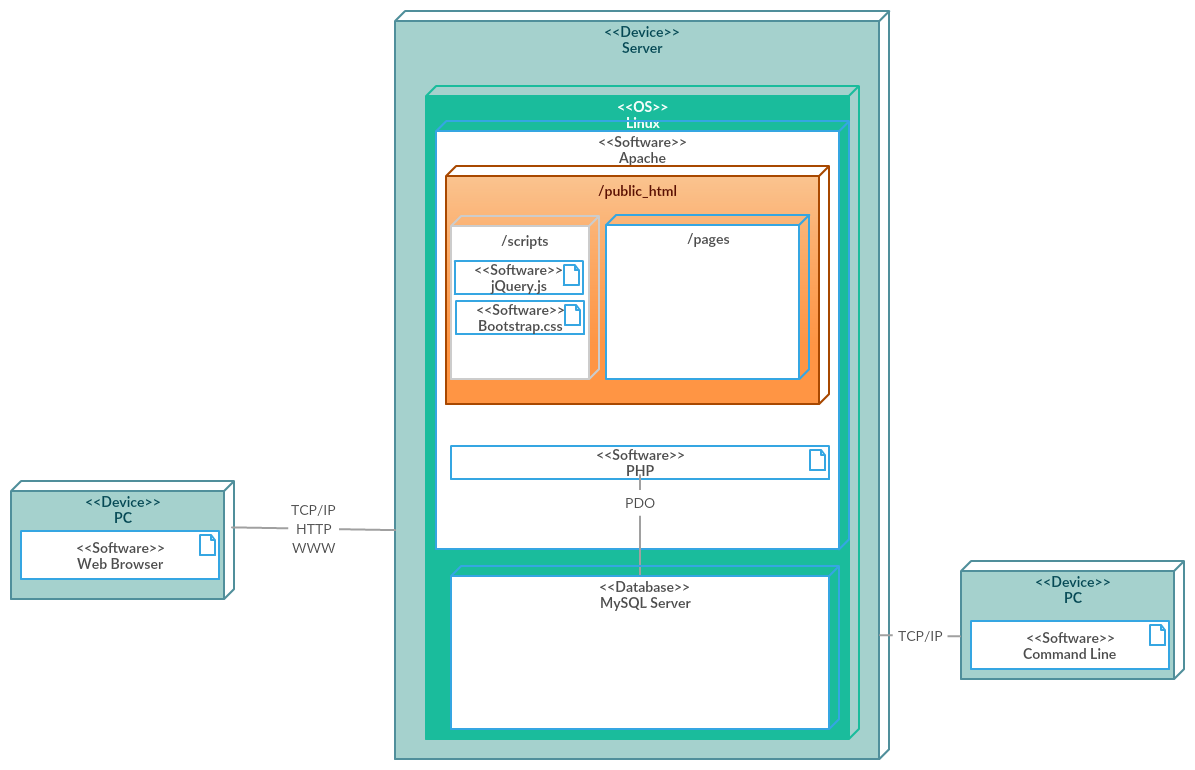
\includegraphics{apps} 
{\bf PC (Web Browser)} - users computer that needs a browser installed and a connection to the internet. \\
{\bf TCP/IP, HTTP, WWW} - data communication protocols that are going to be used to connect to the web server for access to the website(TaskerMAN) and to the database(TaskerSRV). \\
{\bf Server} - details of the serveer which runs on Linux(aber.ac.uk) that has Apache installed(Web Server) with the PHP extension installed to process PHP files. PHP extension makes calls to the MySQL DataBase(TaskerSRV) via PHP PDO Prepared statements. \\
{\bf Public\_html} - place where we put all the files for the website, including scripts and web pages, that can be viewed via browsers.\\
{\bf PC(Command Line)} - has an Internet connection and TaskerCLI installed on to access TaskerSRV. Java program that will need use a email for authorisation to communicate with TaskerSVR  using JDBC with MySQL driver.

\subsection{Application interactions}

\section{INTERACTION DESIGN}
\subsection{Use-cases}
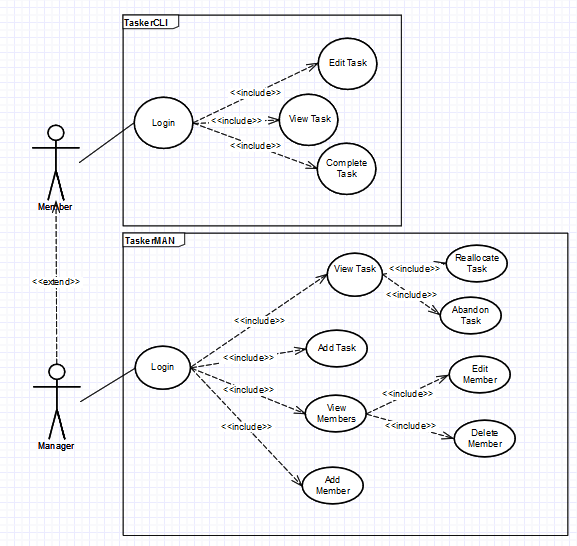
\includegraphics{usecase}

\subsection{User Interface design}

\section{COMPONENT DESCRIPTION}

\section{SIGNIFICANT CLASSES}
\subsection{Interface Description}

\section{DETAILED DESIGN}
\subsection{Sequence diagrams}
\subsection{State diagrams}
\subsection{Activity diagrams}
\subsection{Significant data structures}

\clearpage
\addcontentsline{toc}{section}{REFERENCES}
\begin{thebibliography}{5}
\bibitem{se.qa.03} Nothing yet
\end{thebibliography}
\clearpage

\addcontentsline{toc}{section}{DOCUMENT HISTORY}
\section*{DOCUMENT HISTORY}
\begin{tabular}{|l | l | l | l | l |}
\hline
Version & CCF No. & Date & Changes made to Document & Changed by \\
\hline
0.1 & N/A & 2015-10-20 & Initial creation & OKM \\
\hline
\end{tabular}
\label{thelastpage}
\end{document}
